
\chapter{Aufgabe D6}
Statt der aufgezeichneten Daten werden nun die Geschwindigkeiten aus dem Randomgenerator genutzt, um das Modell zu prüfen. \\
Bei dem Randomgenerator kann die Basisgeschwindigkeit eingestellt werden, die anschließend mit Rauschen, das durch den Randomgenerator generiert wurde, aufaddiert wird. Sowie das Noiselevel/Amplitude, welches das generierte Signal haben soll. Im Folgenden ist ein Ausschnitt zu sehen, wie der Randomgenerator  in das bestehende Modell integriert wird, sowie die erzeugten Daten des Randomgenerators und ob es Imbalancen im System mit dem Randomgenerator gibt.
\begin{figure}[H]
	\centering
	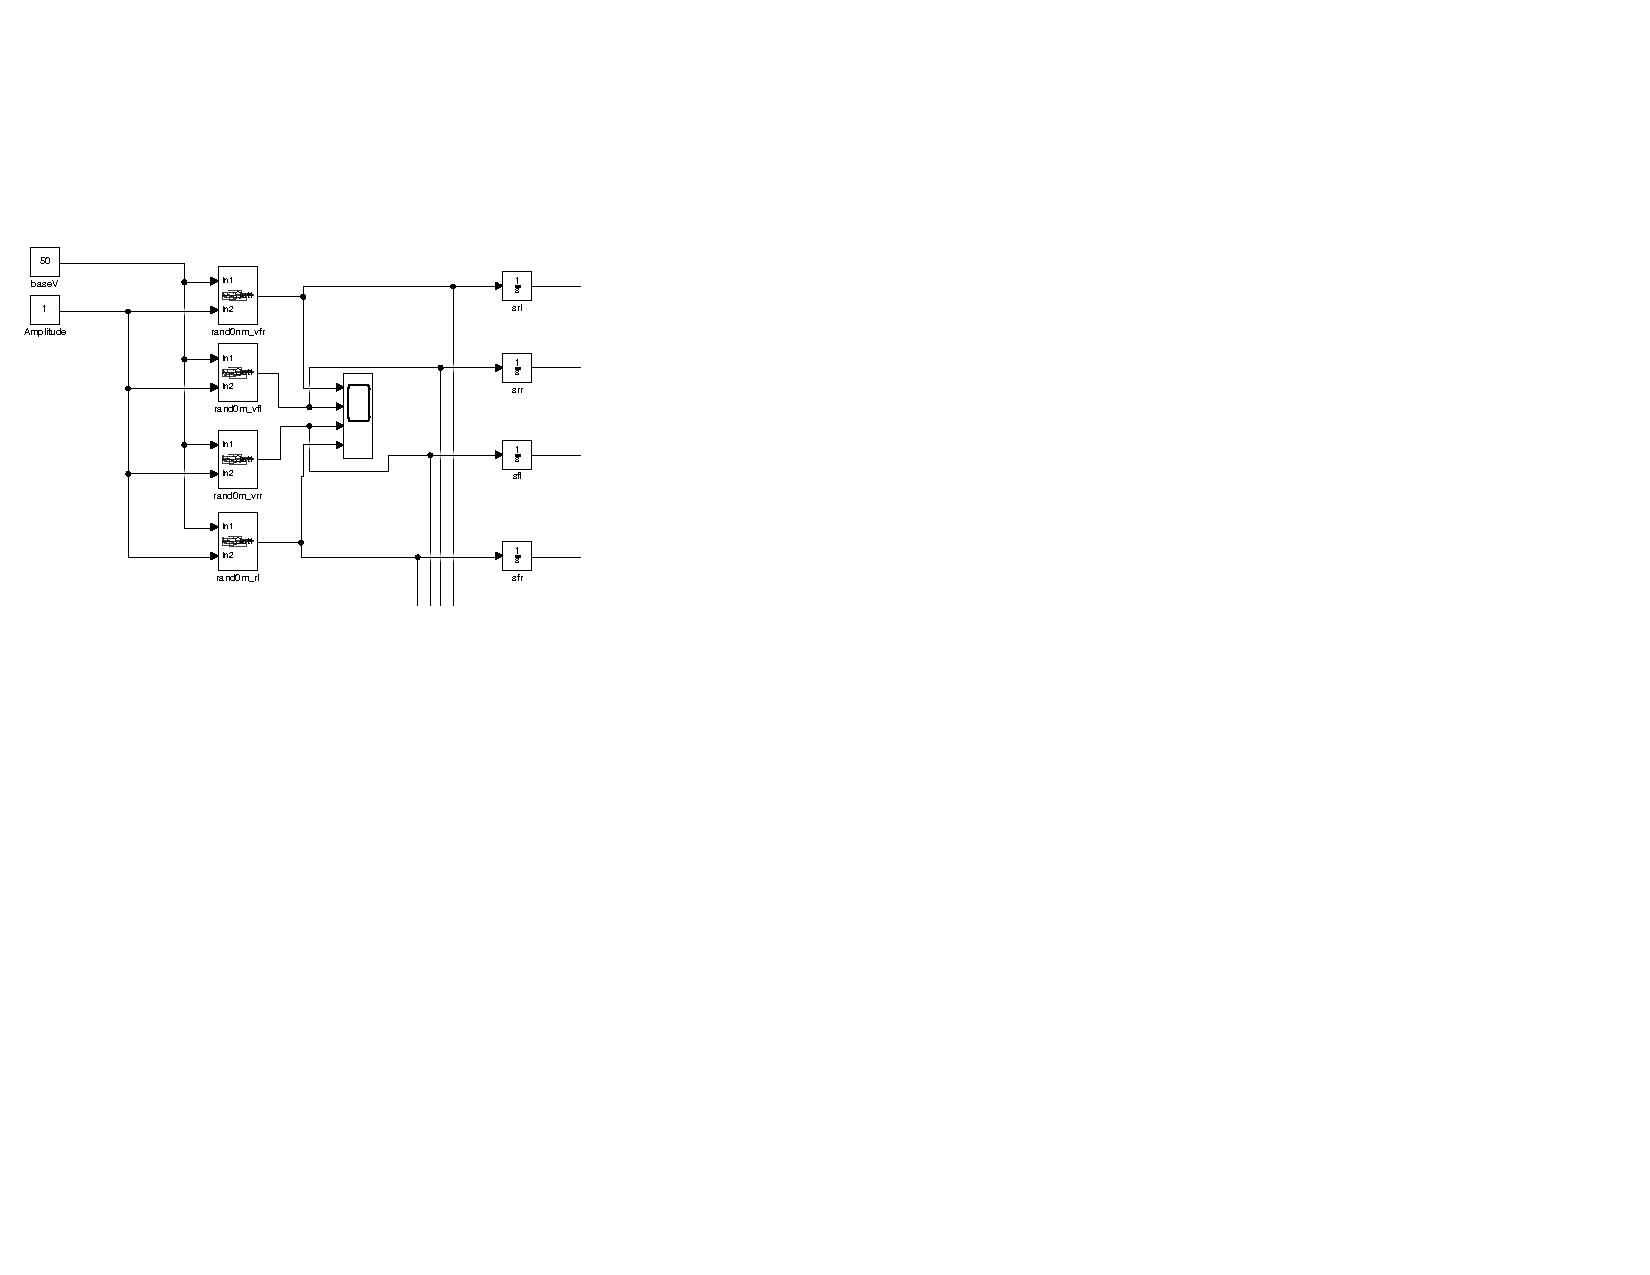
\includegraphics[width=0.95\linewidth]{../Graphiken/TireSimRandom}
	\caption{Include Random Generator}
	\label{fig:randomGeneratorAusschnitt}
\end{figure}
\begin{figure}[H]
	\centering
	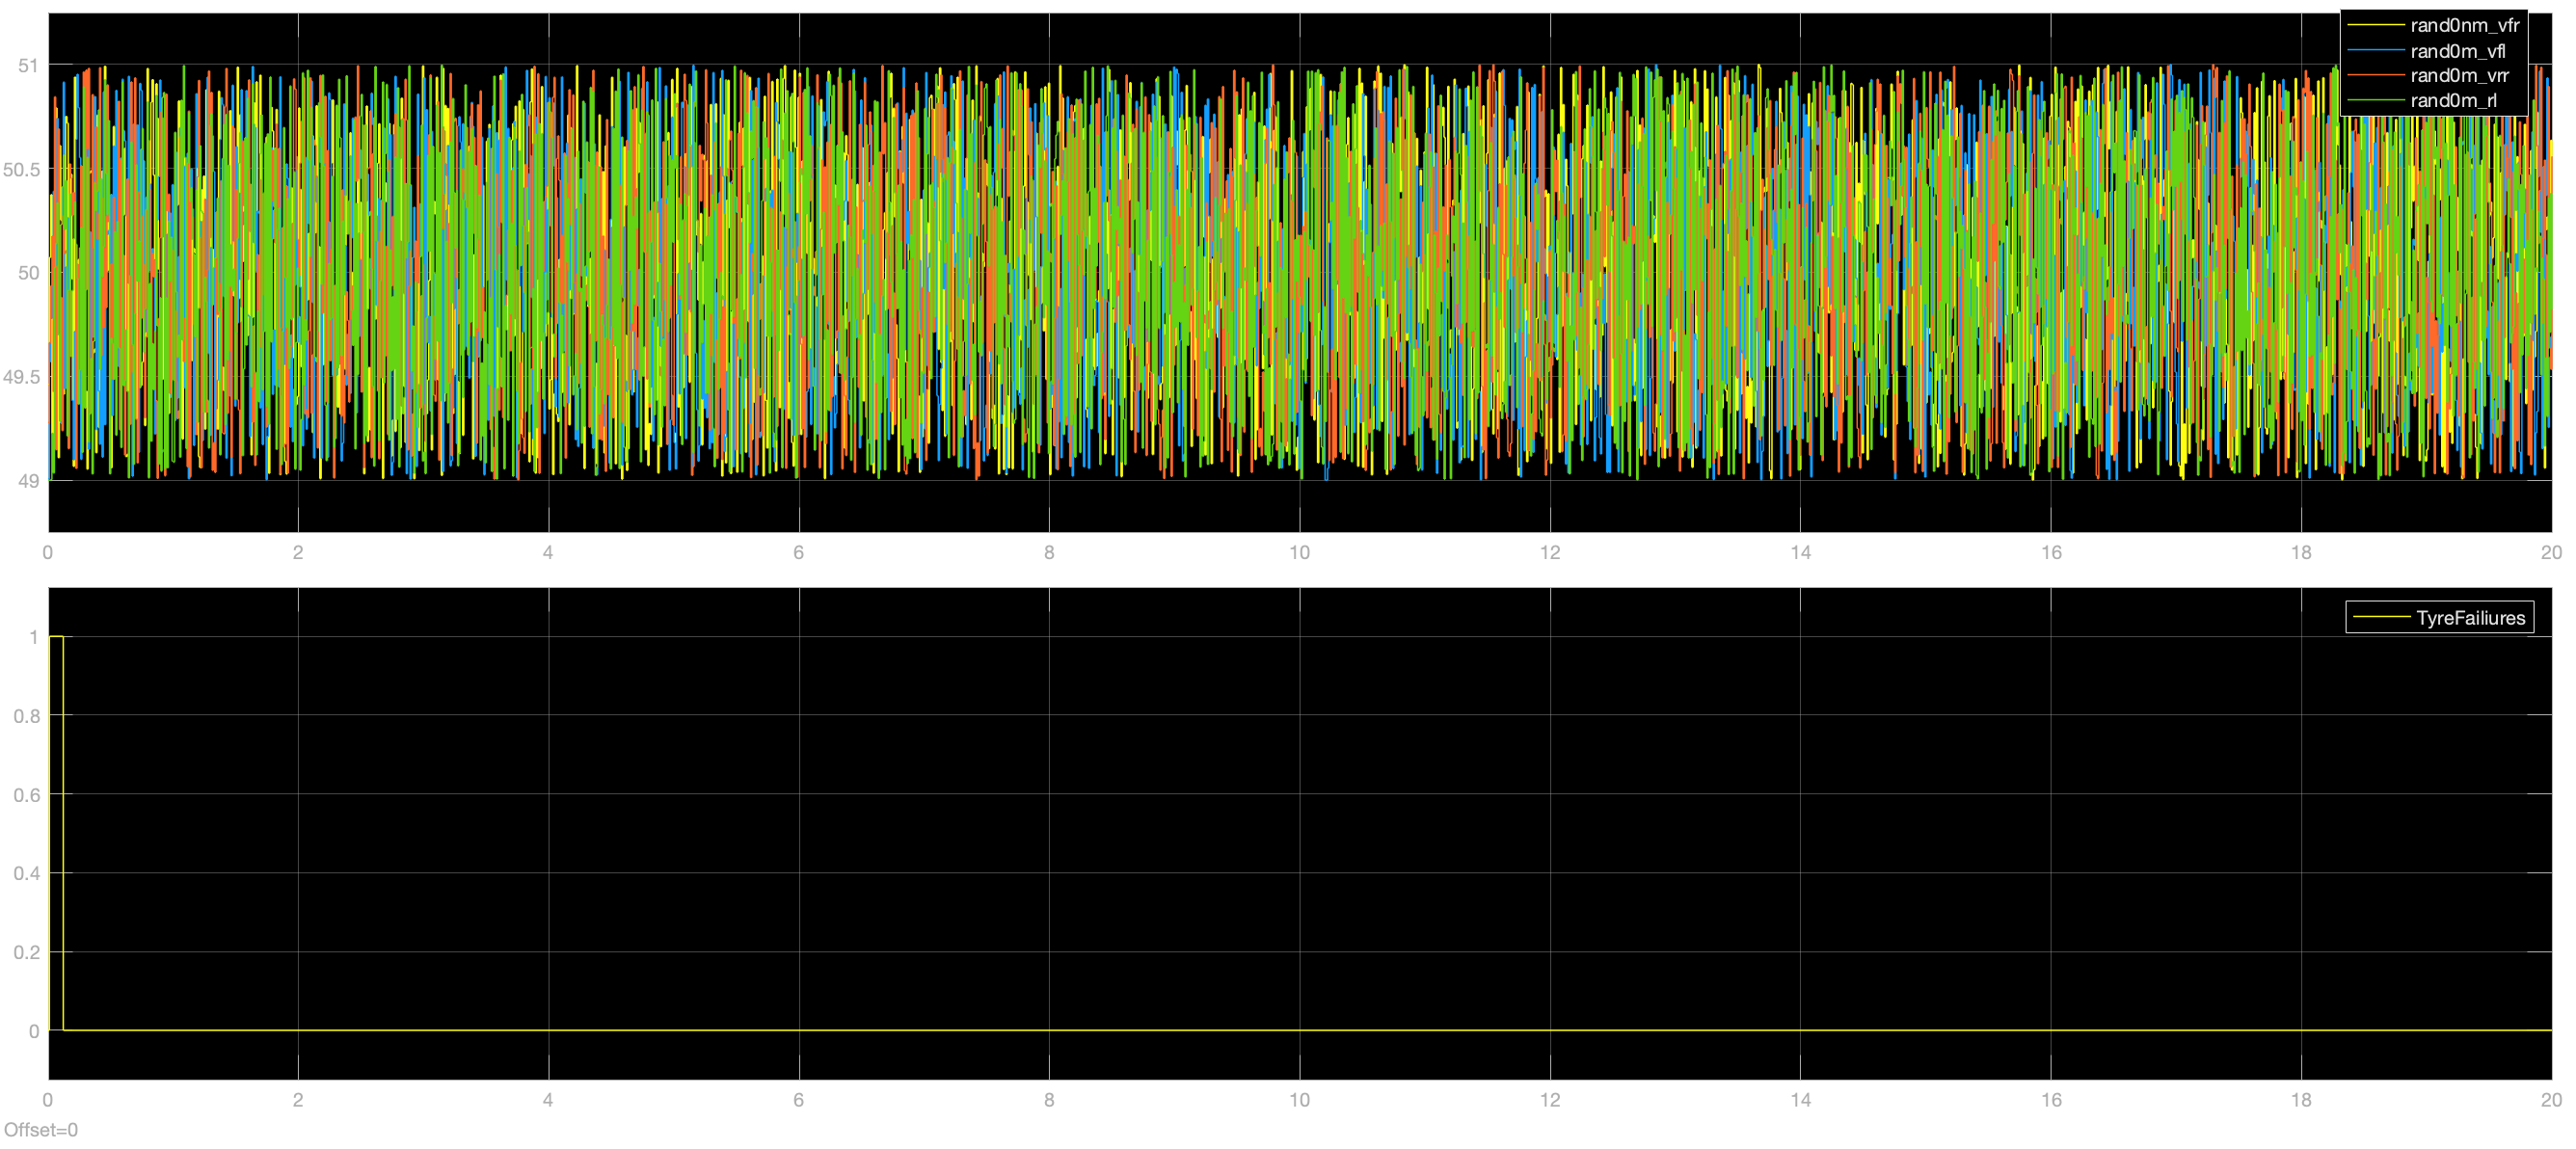
\includegraphics[width=0.95\linewidth]{../Graphiken/RandomGeneratorData}
	\caption{Generated Data}
	\label{fig:randomgeneratordata}
\end{figure}
Es wird deutlich, dass es keine Imbalancen bei diesem Beispiel gibt. Auch bei anderen Basisgeschwindigkeiten und Noiseleveln, die einer realistischen Geradeausfahrt entsprechen, treten keine Imbalancen auf.\\
Damit ist der konstruierte Randomgenerator gut geeignet, um Geradeausfahrten zu simulieren.\\

Wird nun eine Basisgeschwindigkeit so manipuliert, dass die generierte Geschwindigkeit im 10 Sekundendurchschnitt über den 0.5\% liegt, so signalisiert der Tire Monitor eine Reifenimbalance. Als Beispiel haben hier drei Reifen eine Basisgeschwindigkeit von 100km/h, der abweichende Reifen hat eine Basisgeschwindigkeit von 100.7 km/h. Alle Signale Rauschen um 0.5 km/h in die positive und negative Richtung.\\
Im Durchschnitt sollte also eine Geschwindigkeit aller vier Reifen von 100.175 km/h erreicht werden. Die prozentuale Abweichung des abweichenden Reifen ist somit:
$$
\dfrac{|100.175-100.7|}{100.175} = 0.524\%
$$
Der Tire Monitor bestätigt dieses und zeigt eine Imbalance an.
\begin{figure}[H]
	\centering
	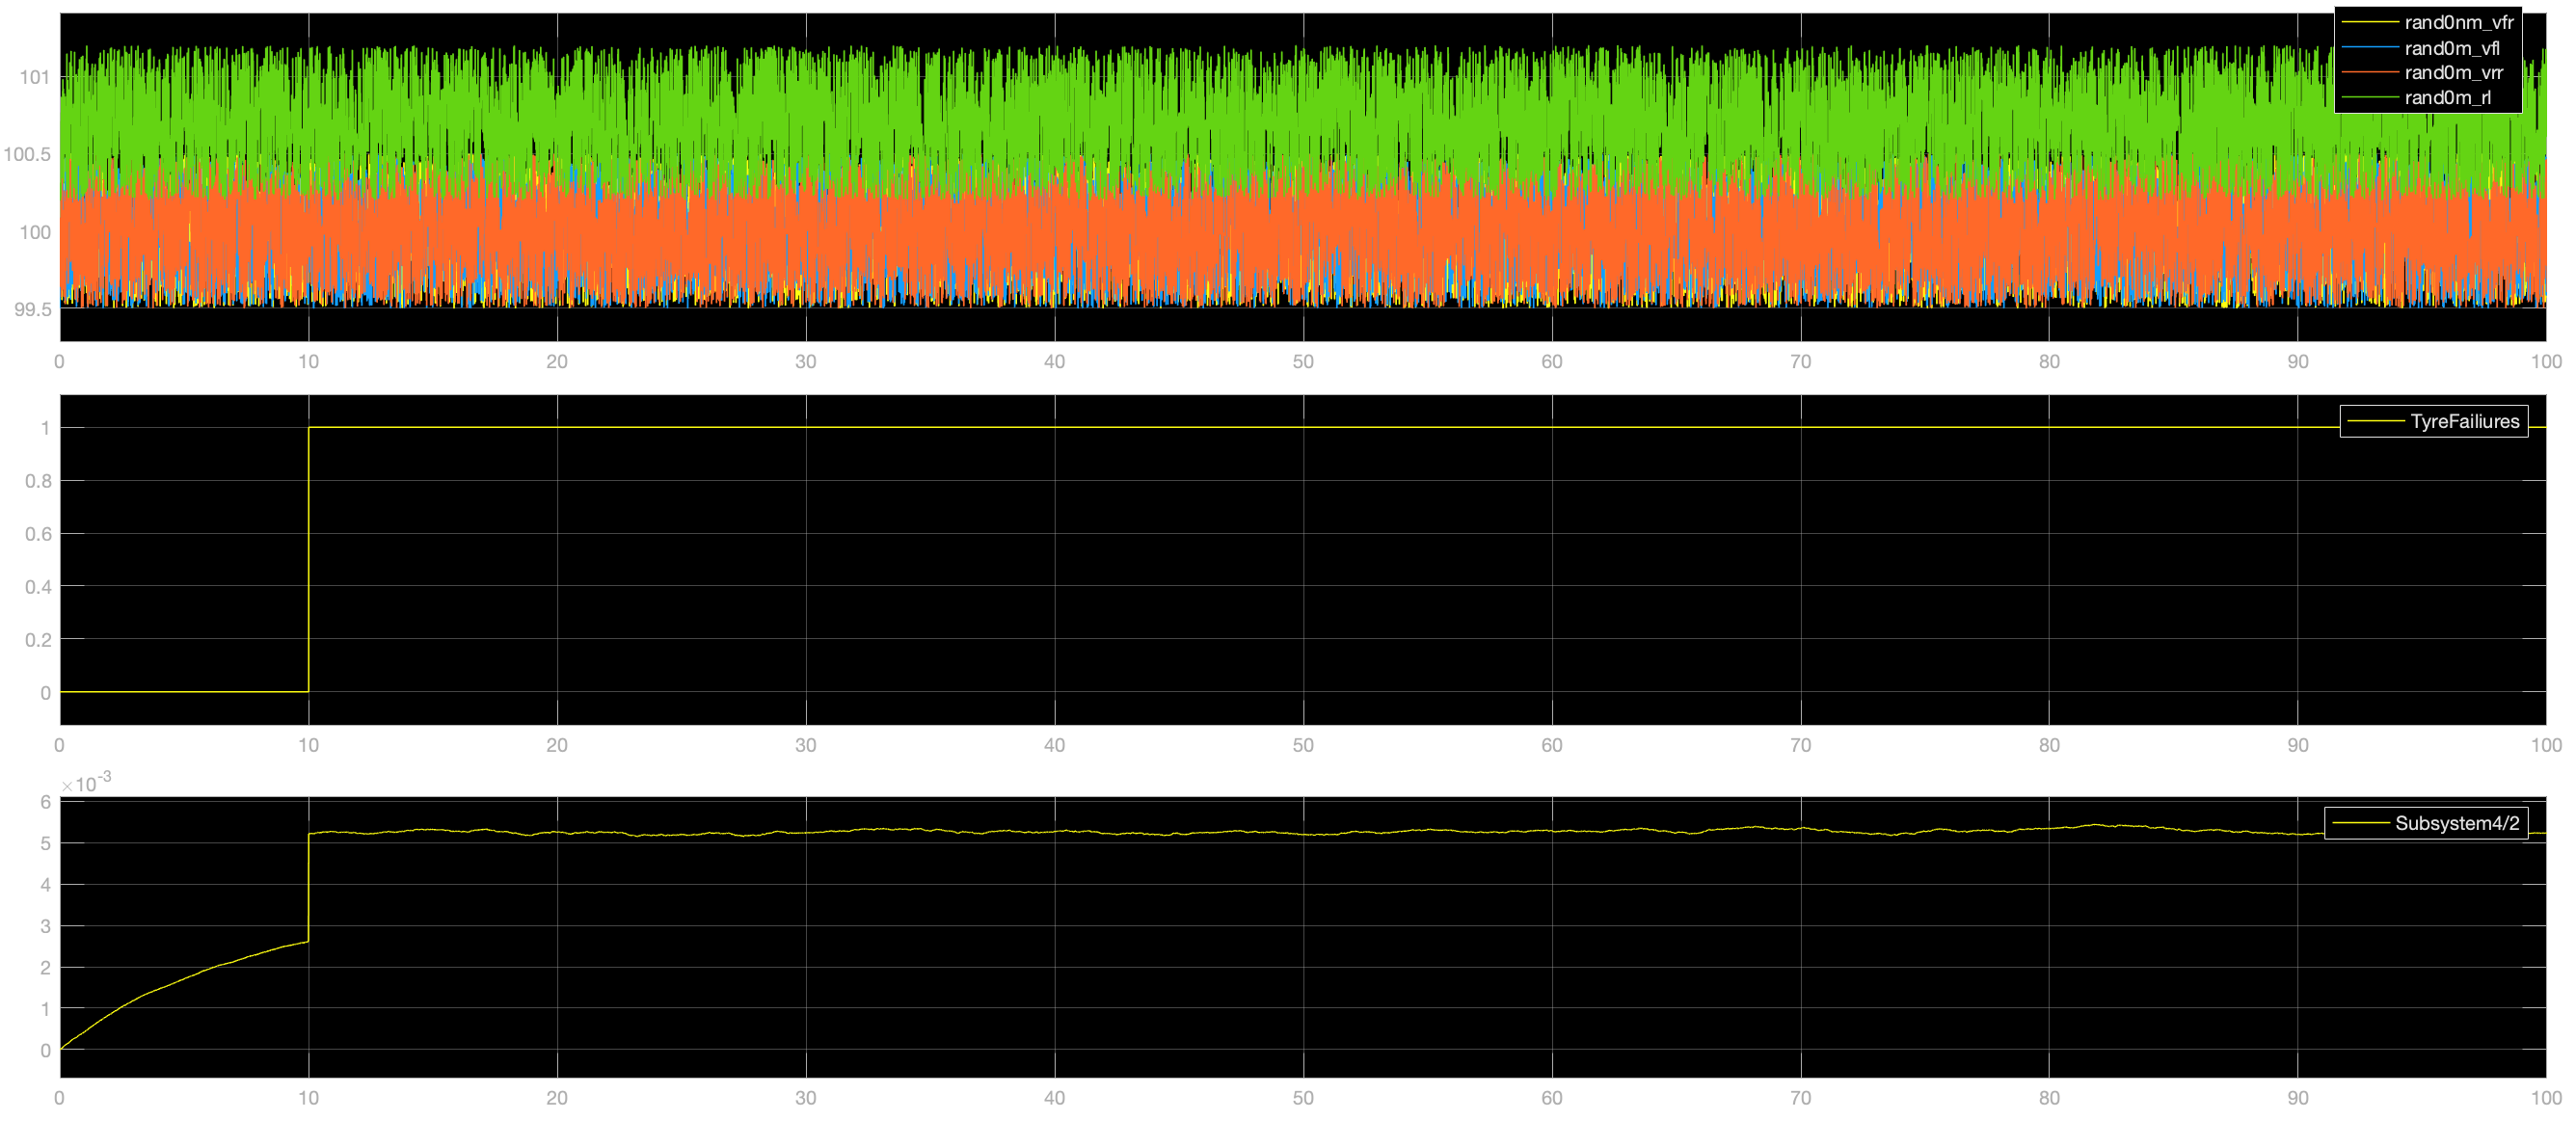
\includegraphics[width=0.95\linewidth]{../Graphiken/RandomAbweichung}
	\caption{Systemtest Funktionalität}
	\label{fig:funkt}
\end{figure}
Der Bereich bis 10s ist bewusst manipuliert wie in D4 angesprochen wurde.
